\documentclass[10pt,a4paper]{article}
\usepackage[utf8]{inputenc}
\usepackage{amsmath}
\usepackage{amsfonts}
\usepackage{amssymb}
\usepackage{graphicx}
\usepackage{placeins}
\author{Bohnstingl Thomas, Scherr Franz}
\title{Autonomously Learning Systems}
\begin{document}
\newcommand{\identity}{\mathbf{I}}
\newcommand{\Xmat}{\mathbf{X}}
\newcommand{\yvec}{\mathbf{y}}
\renewcommand{\th}{\theta}
\newcommand{\dthi}{\frac{\partial}{\partial \th_i}}
\newcommand{\dthj}{\frac{\partial}{\partial \th_j}}
\section{Deep Q-Learning}

We implemented the Q-learning algorithm with experience replay as given in the practical slides. In order to further improve performance, we researched the internet and found a few hints that may help:

\begin{itemize}
  \item Double Q-learning
  \item Duelling Q-learning
  \item Improved Action Selection
\end{itemize}

\subsection{Double Q-learning}
At first, Double Q-learning is the strategy to keep two seperate Q networks to decouple action selection and target Q estimation. This helps to prevent the case that Q values are overestimated. This improvement is already included in the algorithm given in the practical slides.

\subsection{Duelling Q-learning}
A viable approach to improve the Q-learning algorithm is to split up the network in an advantage and a value part. That is:
\begin{align*}
  Q(s, a) &= A(s, a) + V(s)
\end{align*}

The essential point is that the whole network in its entirety will generalize the value of a specific state better and learns the actual advantage of the actions in a different part. This somehow brings the Q-network closer to a policy agent in the sense that the action distribution is located in the advantage part.

Moreover, this also enables us to implement a model based learning technique additionally as we already have a value estimation. For example, consider Markov Tree Search (MCTS). We could readily approach this extension if we have an estimation for the value of a state. Still we would need a part to predict state transitions. However, we did not have sufficient time for this and might consider to poke around with this in the future.

\subsection{Improved Action Selection}
The action selection is an essential part that decides about the distribution of exploiting and exploring. The basic epsilon greedy approach is suboptimal. Possibly a better approach would be to sample the actual action with a probility distribution according to the estimated Q-values. This is given with the Boltzmann distribution where we transform the Q-values to a probability distribution according to:
\begin{align*}
  p(a | s) &= \frac{e^{\frac{Q(s, a)}{T}}}{\sum_{a'} e^{\frac{Q(s, a')}{T}}}
\end{align*}
which is simply a softmax of the Q-values. However, there is a major drawbacks with this approach, that leaded to discard this action selection in more complicated environments compared to CartPole. Since the Q-values reside in very different ranges, it is very hard to choose the right temperature $T$ for the softmax. For example, with CartPole the Q-values would be in range of 0 to 200. And in the case of Pong we had basically a range of -21 to -18 in the beginning. So if we had the same temperature, the probility distributions would be basically random with the Pole environment and extremely sharp in the CartPole environment. In addition, in the ideal case that the network is able to learn and the reward ranges shifts, the action selection strategy would also change its sharpness and in the direction to loose exploration moves. So we stuck with the epsilon greedy approach in the case of Pong, although it worked very well with CartPole.

However, one possibility would be to keep a moving window of the selected actions and compute the ratio of actions selected due to an argmax and explorating actions that were non maximal. We could then proceed to adaptively change the temperature and it would allow to have the exploration weighted with Q-values.

\subsubsection{Exploiting Uncertainty in Action Selection}
It is also conceivable to obtain a better performance if we are able to measure the uncertainty in action selection. Suppose we do, we could simply pick the action that is best within its uncertainty. By playing this action more times, the uncertainty will shrinken and we finally end up exploring a different action that is now more promising within its uncertainty. However, we do not use a probabilistic distribution of network weights but we could do something like that by using dropout. We would sample Q-values several times and compute mean and variance. Then select the action with highest mean plus standard deviation.

\subsection{Convolutional neural network}
To be able to learn from ATARI environments with images as output, a convolutional neural network was implemented. The model was built generic to be able to test various different configurations. The is made of several convolutional layers from the input followed by one or more fully connected layers. Different network configurations with various numbers of filters and filtersizes were tested.
After many unsucessfull trials to train the network on the game pong, the implementation was tested on the MNist data set as proposed in some tensorflow tutorials. A similar network configuration like in the MNist tutorial revealed 99.2\% accuracy.\\

\noindent The configuration for this result was:
\begin{itemize}
\item Two convolutional layers with a filtersize of 5x5
\item The extracted features are 32 and 64
\item Three fully connected layers with 64, 30 and 6 neurons
\end{itemize} 

\noindent After this proof of concept, the same network was trained under supervised conditions for the game pong. Also with this supervised approach the network didn't achieved good results on the ATARI game. Also variations of the network configuration above didn't perform well.\\
After detailed analysis of the issue a problem with the supervised part was detected which will also be discussed in the following section.\\
After the problem with the preprocessing was solved the there was not enough time to train the network on the pong game.

\subsection{Observations and Conclusions}
There were simply too many things to try out and too limited resources.

\subsubsection{Comparing to Policy Gradient in Assignment 3}
The most important conclusion we take from the mini project is that learning Q values of state and actions is much more complicated than learning a policy out from the observations. We suppose that this is because the Q network learns to predict the value of state and actions and therefore tries to model the environment in its network. As opposed to the policy agent, in this case we directly address to learn what actions where appropriate to be taken through a trajectory.

Thus, we had a thinking error that a network about the same size like in assignment 3 would be sufficient. Instead, the Q-network needed a lot more layers to provide reasonable results.

It also has to feature a high nonlinearity which is only achieved through a deep structure. Consider the environment Pong. Suppose the ball is in immediate vicinity of the players racket. Is the ball right about to hit the racket, the network needs to predict a high value and is it about to almost hit the racket but actually does not, the network needs to predict a reward of -1 in this case. This is just a matter of small changes in the observations that have to lead to a very different value.

A policy network learns the probability distribution of actions in this state. Still this distribution has to shift if the ball is about to miss the racket but we would expect that this would not be a similar hard edge as with the Q network.

\subsubsection{Preprocessing}
Since we had a really hard time to train the Q-network for the Pong environment using the preprocessing given in assignment 3, we investigated the preprocessing functions closer. We found that the coordinates are not correct anymore if the ball surpasses a racket. This is because the region to scan for the ball is always in the inner field not considering the outer bands behind the rackets.

We proceeded to implement another preprocessing function that correctly identifies the balls position also if it is behind the rackets. And indeed, we saw a major improvement for the trajectory durations and rewards.

The explanation behind this is that Q-learning updates the model as it sees rewards and propagates them back using the experience buffer that includes nonreward transitions. Because the rewards were given only in the last parts of the trajectory when the observations were not correct anymore, the rewards led the Q-network in the wrong direction. In contrast to policy gradient, the rewards are considered throughout the whole trajectory and associated to what actions the agent has taken throughout it.

\subsection{Results}

\subsubsection{CartPole}
Of course this is the simplest environment. And it turned out that we are indeed easily able to solve it. After about 25 sampled trajectories there is a major turn in reward and we can consider the environment solved after about 40 sampled trajectories. See Figure~\ref{fig:cartpole_reward} that displays the mean rewards over sampled trajectories.

\begin{figure}[!ht]
  \centering
  \includegraphics[width=1\textwidth]{./figures/cartpole_reward.png}
  \caption{Reward in sampled trajectories}
  \label{fig:cartpole_reward}
\end{figure}

\FloatBarrier
\subsubsection{Pong}
As said, the preprocessing was a big obstacle for the Q-network to overcome. In Figure~\ref{fig:deepq_pong_duration} we see that the network was not able to capture the environment. The architecture of the corresponding Q-network was deeper one, because we observed that it slightly improved the rewards. This might be due to the fact that a deeper structure realized in some sense that the observations when the rewards were given were not associated to the actual ball positions anymore.

The structure of the network is also given in Figure~\ref{fig:deepq_relu_structure}. It consisted of several layers of ReLU activated neurons because we came to the conclusion that the sharp transitions in Q-values depending on the position relative to the racket fits the ReLU edge very well.

\begin{figure}[!ht]
  \centering
  \includegraphics[width=1\textwidth]{./figures/long_trial.png}
  \caption{Duration and rewards of episodes with a deep Q network. Computation time: \~6 hours.}
  \label{fig:deepq_pong_duration}
\end{figure}

\begin{figure}[!ht]
  \centering
  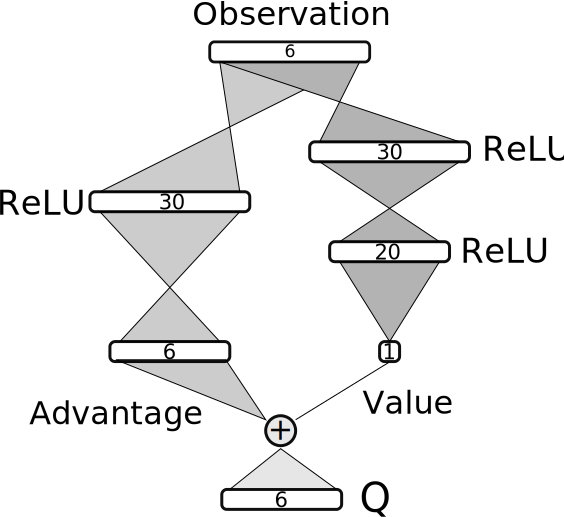
\includegraphics[width=0.5\textwidth]{./figures/deep_relu.png}
  \caption{Structure of the deeper Q-network model}
  \label{fig:deepq_relu_structure}
\end{figure}

\FloatBarrier

The situation was quite different with the improved feature extraction. We again trained a model with the same configuration as above and experienced a much better reward within less iterations. Consider Figure~\ref{fig:deep_corrected} for the rewards and durations.

\begin{figure}[!ht]
  \centering
  \includegraphics[width=1\textwidth]{./figures/relu_corrected.png}
  \caption{Duration and rewards with the same network as given in Figure~\ref{fig:deepq_relu_structure} with corrected features.}
  \label{fig:deep_corrected}
\end{figure}

However, we suppose that in this case the structure is again to complicated for the environment if we got the features right.
\end{document}
